\documentclass[a4paper,10pt]{article}
\usepackage[utf8]{inputenc}
\usepackage[]{polski}
\usepackage{a4wide}
\usepackage{caption}
\usepackage{float}
\usepackage{amsthm}
\usepackage{graphicx}
\usepackage[T1]{fontenc}
\usepackage{listings}
\usepackage{multirow}
\usepackage{longtable}
\usepackage{algorithm}
%\usepackage{algorithmic}
\usepackage{algpseudocode}
\usepackage{enumerate}
\usepackage{booktabs}

\newtheorem{twr}{Twierdzenie}
\newtheorem{lem}[twr]{Lemat}

\title{{\textbf{Grafy i Sieci}}\\[1ex]
       {\Large Sprawozdanie 3}\\[-1ex]
       {\Large Projekt - Graf częściowo spójne}}
\author{Krzysztof Opasiak, Adrian Brzozowski}

% Kropka po numerze paragrafu, podparagrafu itp.
\makeatletter
	\renewcommand\@seccntformat[1]{\csname the#1\endcsname.\quad}
	\renewcommand\numberline[1]{#1.\hskip0.7em}
\makeatother

% Kropka po numerze tablicy, rysunku i ustawienie czcionki dla etykiety.
\captionsetup{labelfont=sc,labelsep=period}

% Numeracja wzorów według paragrafu.
\renewcommand{\theequation}{\arabic{section}.\arabic{subsection}.\arabic{subsubsection}}

%\renewcommand{\thesubsection}{\alph{subsection}}
%\renewcommand{\thesubsubsection}{\Roman{subsubsection}}

% Zmiana nazwy figure "Rysunek" -> "Wykres"
\renewcommand{\figurename}{Wykres}

% Środowisko definition z numeracją
\newtheorem{definition}{Definicja}
\newtheorem{theorem}{Twierdzenie}

\date{Warszawa, \today r.}
\begin{document}
\maketitle

\section{Testy}
\subsection{Sprawdzenie poprawności}

Poprawność zaimplementowanego algorytmu wykazano na podstawie ręcznego przeliczenia uprzednio przygotowanych grafów.\\

Testy wykonywane były wedle następujących kroków:
\begin{enumerate}
\item Wygenerowanie garfu
\item Wyznaczenie ręczne składowych częściowo spójnych danego grafu
\item Uruchomienie algorytmu wyznaczającego składowe częściowo spójne
\item Porównanie wyników
\end{enumerate}

\subsection{Testy deterministyczne}
\subsubsection{Wyniki testów}

\begin{center}
\begin{tabular}{|l|c|l|l|}\hline
{\bf Dane wejściowe}&{\bf Graf}&{\bf Dane wyjściowe}&{\bf Test}\\ \hline
\shortstack[l]{
5\\
1 2 3 4\\
0 2 3 4\\
0 1 3 4\\
0 1 2 4\\
0 1 2 3
}
&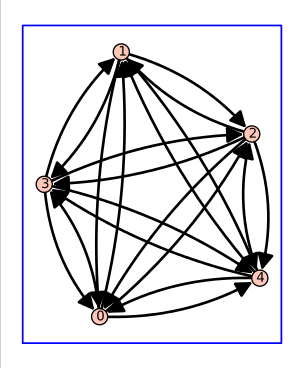
\includegraphics[width=5 cm]{sample_data}&
\shortstack[l]{
1\\
0 1 2 3 4 
}
&OK\\ \hline
\end{tabular}
\end{center}

\begin{center}
\begin{tabular}{|l|c|l|l|}\hline
{\bf Dane wejściowe}&{\bf Graf}&{\bf Dane wyjściowe}&{\bf Test}\\ \hline
\shortstack[l]{
5\\
1 2 3\\
2 3 4\\
0 1 3\\
0 2 4\\
0 1 2
}
&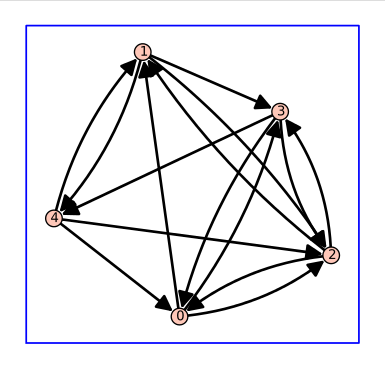
\includegraphics[width=5 cm]{sample_data2}&
\shortstack[l]{
1\\
0 1 2 3 4 
}
&OK\\ \hline

\shortstack[l]{
9\\
6\\
4\\
8\\
0\\
7\\
7 2\\
8 3\\
1\\
5
}
&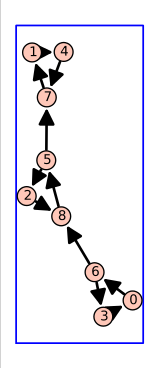
\includegraphics[height=6 cm]{sample_data3}&
\shortstack[l]{
1\\
0 6 3 5 2 8 1 4 7 
}
&OK\\ \hline

\shortstack[l]{
10\\
2 4 6 8\\
3 5 7 9\\
4 6 8 0\\
5 7 9 1\\
6 8 0 2\\
7 9 1 3\\
8 0 2 4\\
9 1 3 5\\
0 2 4 6\\
1 3 5 7
}
&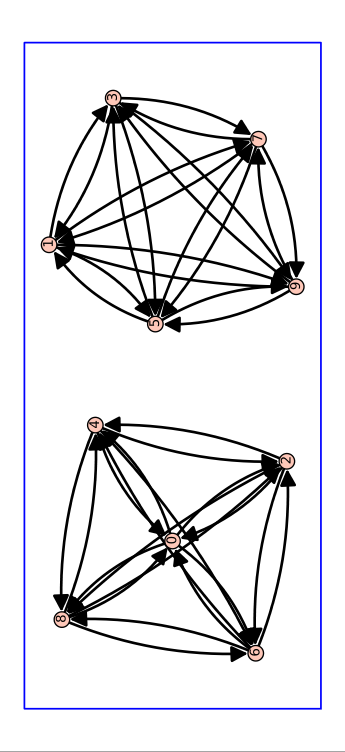
\includegraphics[width=5 cm]{sample_data4}&
\shortstack[l]{
2\\
1 3 5 7 9\\
0 2 4 6 8 
}
&OK\\ \hline
\end{tabular}
\end{center}

\begin{center}
\begin{tabular}{|l|c|l|l|}\hline
{\bf Dane wejściowe}&{\bf Graf}&{\bf Dane wyjściowe}&{\bf Test}\\ \hline
\shortstack[l]{
5\\
4\\
0 2\\
0 1 3\\
0\\
3
}
&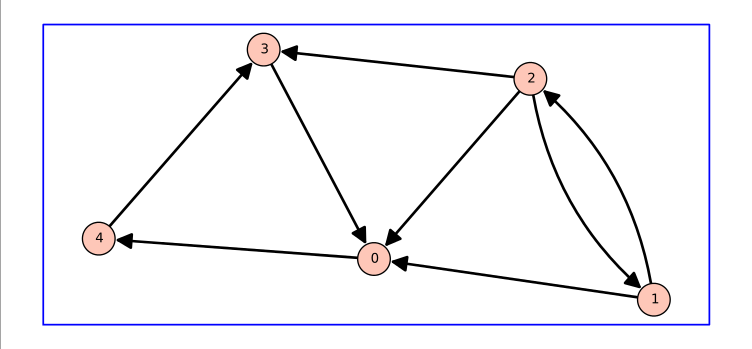
\includegraphics[width=5 cm]{sample_data5}&
\shortstack[l]{
1\\
1 2 0 4 3 
}
&OK\\ \hline

\shortstack[l]{
8\\
4\\
0 2 4\\
3 7\\
2 7\\
0\\
4 6\\
7\\
7
}
&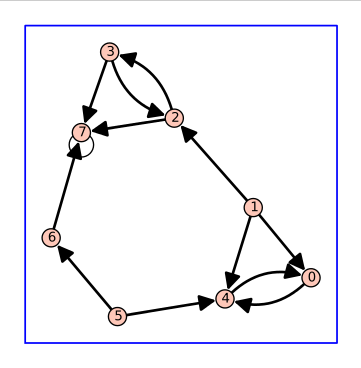
\includegraphics[width=5 cm]{sample_data6}&
\shortstack[l]{
4\\
5 0 4\\
5 6 7\\
1 0 4\\
1 2 3 7 
}
&OK\\ \hline

\shortstack[l]{
4\\
1 2\\
3\\
1 3\\
3
}
&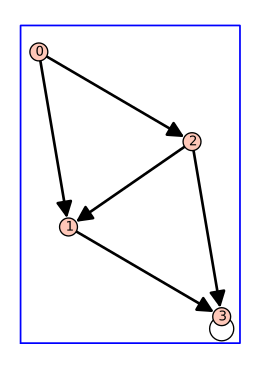
\includegraphics[width=3 cm]{sample_data7}&
\shortstack[l]{
1\\
0 2 1 3
}
&OK\\ \hline

\shortstack[l]{
6\\
3\\
2 5\\
3\\
5\\
1\\
4
}
&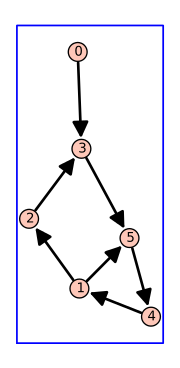
\includegraphics[width=3 cm]{sample_data8}&
\shortstack[l]{
1\\
0 1 2 3 5 4 
}
&OK\\ \hline

\shortstack[l]{
7\\
3\\
0\\
4\\
5\\
5\\
1\\
1 2
}
&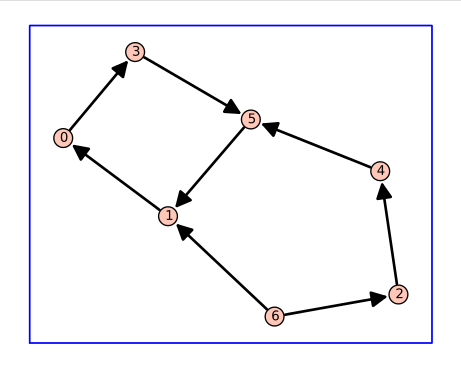
\includegraphics[width=3 cm]{sample_data9}&
\shortstack[l]{
1\\
6 2 4 0 3 5 1 
}
&OK\\ \hline

\shortstack[l]{
4\\
3\\
3\\
3\\
0
}
&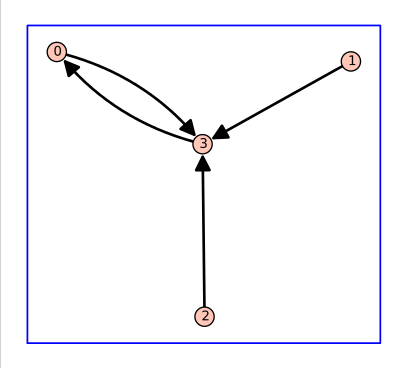
\includegraphics[width=3 cm]{sample_data10}&
\shortstack[l]{
2\\
2 0 3\\
1 0 3 
}
&OK\\ \hline

\end{tabular}
\end{center}

\subsubsection{Wnioski}
Na podstawie powyższych wyników można stwierdzić poprawność działania algorytmu. Tym samym stwierdzamy, że wyznaczane prze algorytm składowe częściowo spójne spełniają warunek bycia poprawną składową częściowo spójną.

\subsection{Testy niedeterministyczne}

W tej części testów wymagane było napisanie programu generującego losowe grafy. Na podstawie wybranej próbki 5 grafów stwierdzono poprawność generowania składowych częściowo spójnych.\\

Do testów posłużyły następujące grafy:
\begin{center}
\begin{tabular}{|l|c|l|l|}\hline
{\bf Dane wejściowe}&{\bf Graf}&{\bf Dane wyjściowe}&{\bf Test}\\ \hline

\shortstack[l]{
7\\
2 3 4 \\
3 1 \\
1 6 \\
2 \\
6 0 \\
3 
}
&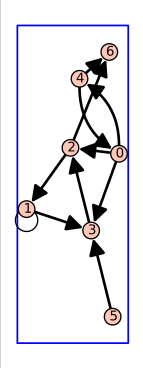
\includegraphics[height=6 cm]{graph_7_11}&
\shortstack[l]{
2\\
5 1 3 2 6 \\
0 4 1 3 2 6 
}
&OK\\ \hline

\shortstack[l]{
8\\
3 \\
\\
4 6 0 \\
4 \\
7 \\
\\
2 \\
1 
}
&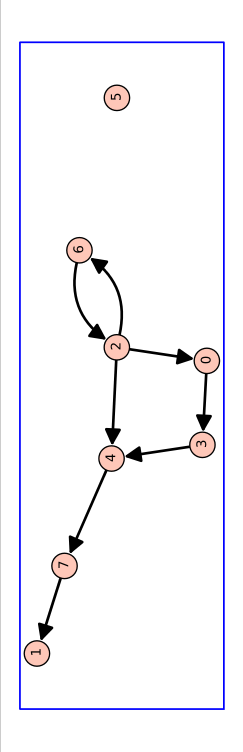
\includegraphics[height=6 cm]{graph_8_8}&
\shortstack[l]{
2\\
5 \\
2 6 0 3 4 7 1 
}
&OK\\ \hline

\end{tabular}
\end{center}

\begin{center}
\begin{tabular}{|l|c|l|l|}\hline
{\bf Dane wejściowe}&{\bf Graf}&{\bf Dane wyjściowe}&{\bf Test}\\ \hline

\shortstack[l]{
9\\
7 \\
\\
8 \\
8 \\
7 \\
8 \\
\\
7 \\
8 
}
&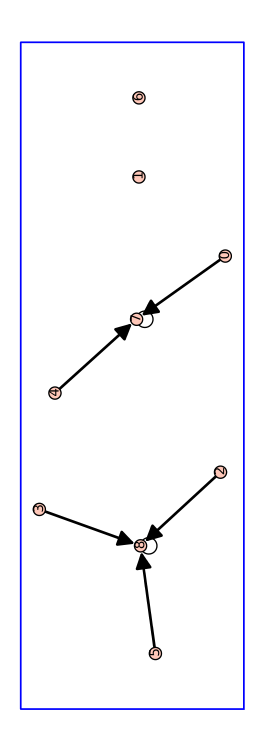
\includegraphics[height=6 cm]{graph_9_7}&
\shortstack[l]{
7\\
6 \\
5 8 \\
4 7 \\
3 8 \\
2 8 \\
1 \\
0 7 
}
&OK\\ \hline

\shortstack[l]{
9\\
7 \\
8 5 \\
8 3 \\
8 6 3 \\
7 3 \\
8 1 5 \\
2 \\
7 \\
8 2 8 
}
&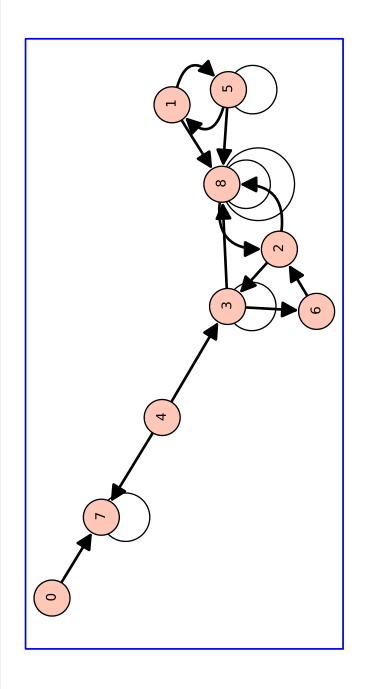
\includegraphics[width=3 cm]{graph_9_18}&
\shortstack[l]{
3\\
4 2 3 6 7 \\
1 5 7 \\
0 7 
}
&OK\\ \hline

\shortstack[l]{
10\\
4 \\
3 7 \\
0 9 7 \\
4 2 5 \\
7 0 \\
5 \\
8 \\
3 3 \\
5 4 9 \\
4 7 
}
&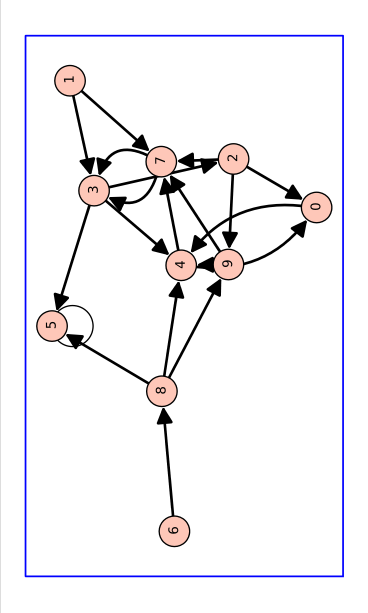
\includegraphics[width=3 cm]{graph_10_20}&
\shortstack[l]{
2\\
6 8 0 4 7 3 2 9 5 \\
1 0 4 7 3 2 9 5 
}
&OK\\ \hline

\end{tabular}
\end{center}

\subsection{Określenie złożoności czasowej algorytmu}
Do określenia złożoności czasowej algorytmu napisano:

\begin{enumerate}
\item Program do generowania losowych grafów
\item Skrypt generujący zadaną próbkę grafów
\item Skrypt wykonujący testy złożoności czasowej algorytmu
\end{enumerate}

Złożoność algorytmiczną wyznaczono na podstawie 7343 próbek.\\
Dane maszyny na której dokonywano obliczeń:

\begin{itemize}
\item Architecture: $x86\_64$
\item CPU op-mode(s): $32-bit, 64-bit$
\item CPU(s): 2
\item Vendor ID: GenuineIntel
\item Model name: Pentium(R) Dual-Core CPU T4500 @ 2.30GHz
\end{itemize}

Na systemie: Linux $3.15.7-1-ARCH x86\_64 GNU/Linux.$ \\

Program do generowania grafów zawiera się w poniższym algorytmie:

\begin{algorithm}
\caption{Generowanie grafów}
\begin{algorithmic}
\State $number\_edges$
\State $number\_vertices$
\Function{generate\_graph}{G}
\While{true}
\For{v in verticles(G)}
	\For{v in verticles(G)}
	  \If{  $rand() \bmod\; 2 == 1$}
    	\State $create\_edge\_to$ $rand()\bmod\; number\_vertices$
    	  \State $++t $
	  \If{$ t == number\_edges$}
    	  \State $end $    	  
	  \EndIf      	  
	  \EndIf  
	\EndFor
\EndFor
\EndWhile
\EndFunction
\end{algorithmic}
\end{algorithm}

Umożliwia on generowanie grafów o zadanej liczbie wierzchołków oraz krawędzi, generując także wszystkie grafy mniejsze tz. z mniejszą liczbą wierzchołków oraz krawędzi.

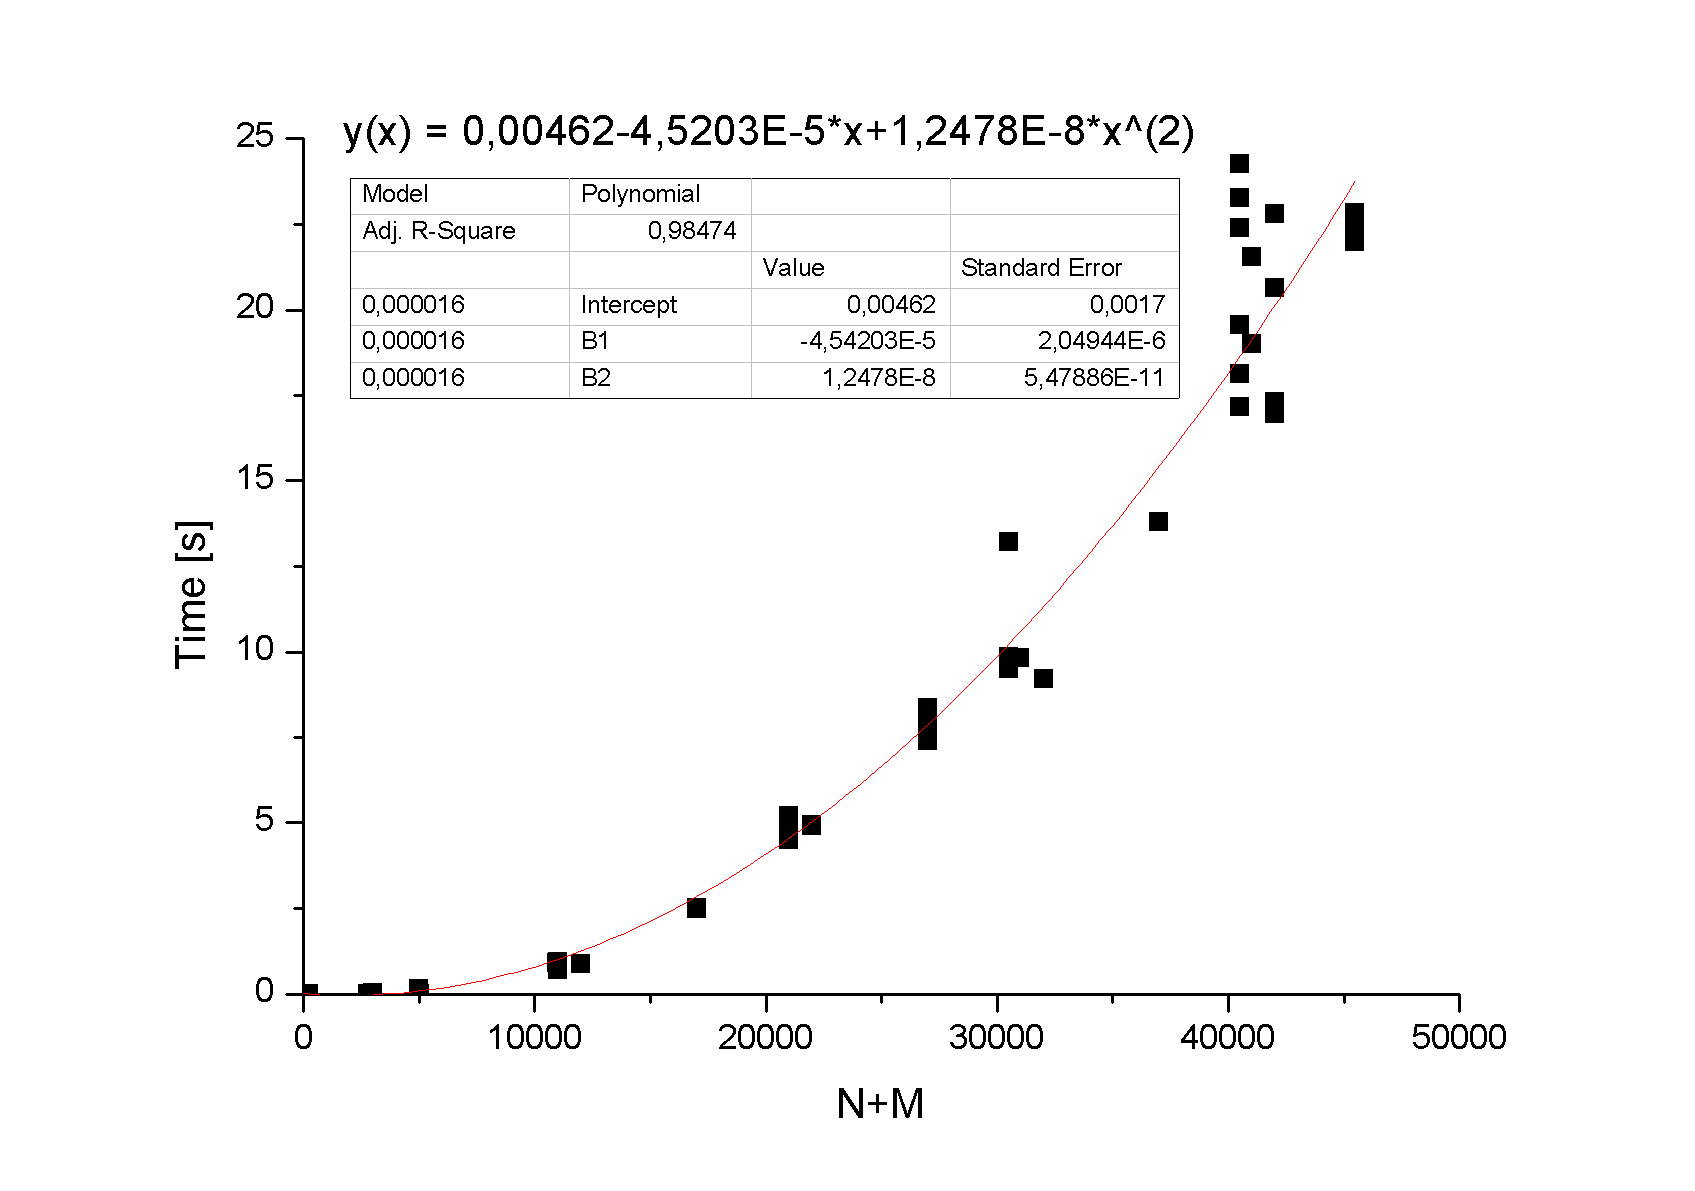
\includegraphics[width=12 cm]{Graph1}


Powyższy wykres ukazuje rozkład próbek,w zależności od liczby krawędzi plus liczba wierzchołków danego grafu do czasu przetwarzania danego grafu w celu wyznaczenia jego składowych częściowo spójnych.\\

Uwidocznia się tutaj złożoność wielomianowa zaimplementowanego algorytmu. Stwierdzono, że najlepszym przybliżeniem będzie wielomian drugiego stopnia, którego wzór ma następującą postać:
$$
y(x) = 0,00462-4,5203E-5*x+1,2478E-8*x^2
$$

\end{document}

\begin{thebibliography}{9}
\bibitem{Cormen} T.H. Cormen, C.E. Leiserson, R.L. Rivest, \emph{Wprowadzenie do algorytmów}, Wydawnictwo Naukowo-Techniczne, Warszawa 2001.
\end{thebibliography}
\end{document}

